% File SDSS2020_SampleExtendedAbstract.tex
\documentclass[10pt]{article}
\usepackage{sdss2020} % Uses Times Roman font (either newtx or times package)
\usepackage{url}
\usepackage{latexsym}
\usepackage{amsmath, amsthm, amsfonts}
\usepackage{algorithm, algorithmic}  
\usepackage{graphicx}

\title{Sparse Bayesian Predictive Modelling of Tumor Response 
	from Radiomic Data}

\author{
  Shirin Golchi\\
  Department of Biostatistics\\ McGill University \\
  Purvis Hall, 1020 Pine Ave W\\
  Montreal QC H3A 1A2 \\ 
  {\tt shirin.golchi@mcgill.ca} \\\And
  Reza Forghani \\
  Department of Diagnostic Radiology \\ McGill University \\
  1650 Cedar Avenue \\
  Montreal QC H3G 1A4 \\
  {\tt reza.forghani@mcgill.ca} \\\And
  Sahir Bhatnagar \\
  Department of Biostatistics\\ Department of Diagnostic Radiology \\ McGill University \\
  Purvis Hall, 1020 Pine Ave W\\
  Montreal QC H3A 1A2 \\
  {\tt sahir.bhatnagar@mcgill.ca} 
}
  

\date{}

\begin{document}
\maketitle
\begin{abstract}
We propose a Bayesian hierarchical model for the analysis of radiomic data for characterization of head and neck squamous cell carcinoma (HNSCC). The proposed model facilitates radiomic feature selection, dealing with missing values in key predictors as well as prediction in a unified framework. 


\end{abstract}

{\bf Keywords:} Radiomics, Multilevel Modeling, Horseshoe prior, Missing Data

\section{Introduction}

An important objective in oncology is the creation of a standardized set of criteria to predict and monitor tumor response to treatment and for outcome prognosis based on objectively measured biomarkers. In addition to the traditional role of imaging for staging and post treatment follow-up of HNSCC, there is increasing interest in the use of quantitative image extracted or radiomic features for characterization of HNSCC. Image analysis algorithms extract mathematically defined features of the tumor's appearance giving rise to high-dimensional matrix covariates. 

Many challenges arise from the structure of radiomic data. Namely, an efficient and reliable variable selection technique is required to select a reasonable number of radiomic features to be used in prediction of key outcomes such as lymph node metastasis. Variable selection and prediction should reflect the heterogenity among tumor sites, however, site-stratified inference can result in low statistical power. In addition, there is a considerable amount of missing data among important predictors such as the presence/absence of human papilloma virus (HPV). 

We propose a Bayesian hierarchical model that can address radiomic feature selection and prediction in a unified framework while dealing with complexities such as missing values in predictors. The hierarchical nature of the model enables information borrowing across tumor sites while allowing site-specific variable selection and parameter estimation. Integrating variable selection and missing data handling together with inference, results in predictions with adequate representation of uncertainty associated with each of these procedures. We present the results of the analysis as Bayesian feature selection outcomes across sites and the accuracy for predictions of lymph node metastasis.

\section{Methods}

Below we describe a Bayesian hierarchical model that takes advantage of regularized horseshoe priors \cite{PiiVeh2017} to perform site-specific radiomic feature selection while borrowing information across sites.  Let $y_{1n}$ and $y_{2n}$ denote the binary outcomes lymph node metastasis and HPV for patient $n = 1, \ldots, N$, respectively. While HPV may be predicted by a number of covariates such drinking and smoking habits, it is an important predictor for lymph node metastasis. Therefore, we define the model as follows,
\begin{equation}
\label{eqn:model}
y_{1n} \sim \text{Bernoulli}(\pi_{1n}),\hskip 10pt y_{2n} \sim \text{Bernoulli}(\pi_{2n})
\end{equation}
where,
\begin{equation*}
\text{logit}(\mathbf{\pi}_{1n}) = \phi \pi_{2n} + \mathbf{z}_n \boldsymbol{\eta}_1+ \mathbf{x}_n\boldsymbol{\beta}_{1s_n}, \hskip 20pt n = 1, \ldots,N
\end{equation*}
where $\pi_{2n}$ is the risk of HPV for patient $n$ that is in turn modelled as,
\begin{equation*}
\text{logit}(\pi_{2n}) = \mathbf{z}_n \boldsymbol{\eta}_2+ \mathbf{x}_n\boldsymbol{\beta}_{2s_n}, \hskip 20pt n = 1, \ldots,N
\end{equation*}
where $s_n = 1,\ldots, S$ are the tumor site, $ \mathbf{z}_n$ are the set of covariates (drinking, smoking and T-stage group)  and  $\mathbf{x}_n$ is the $F\times 1$ vector of radiomic features for patient $n$.

Allowing for the feature selection to be performed separately across the three sites introduces $F\times S$ coefficients. The notation $\boldsymbol{\beta}_{s_n}$ is used to represent the site-specific set of the radiomic feature coefficients matrix.

Following \cite{PiiVeh2017} the coefficients, $\beta_j$, $j = 1, \ldots, J$, of the radiomic features are assigned the following prior distribution,
\begin{align*}
&\beta_{j,s_n} \sim \mathcal{N}(0, \tau^2_{s_n}\tilde{\lambda}_j^2)\\
& \tilde{\lambda}_j^2 = \frac{c^2\lambda_j^2}{c^2 + c^2\lambda_j^2}
\end{align*}
where 
\begin{align*}
&\lambda_j \sim \mathcal{C}^+(0,1),\\
& c^2\sim \mathcal{IG}(\frac{\nu}{2},\frac{\nu}{2}s^2),\\
& \tau_{s_n} \sim \mathcal{C}^+(0, \tau_0).
\end{align*}
where $\nu = 20$, $s^2 = 4$ and $\tau_0=0.001$. These values are chosen according to recommendations in \cite{PiiVeh2017}. Note the subscript $s_n$ for parameter $\tau$ that represents the site specific variance for $\beta_{j,s_n}$. 

As mentioned earlier, a considerable portion of the patients have a missing HPV outcome. The above model is dealing with this issue by augmenting the HPV data with the unknown values of HPV and estimating the missing values together with the rest of the model parameters. 

The inference relies on the posterior distribution of parameters of interest, i.e., $(\phi, \boldsymbol{\eta}_1, \boldsymbol{\eta}_2, \boldsymbol{\beta}_{1s_n}, \boldsymbol{\beta}_{2s_n})$. Sampling from the posterior is performed using Stan.

\section{Data/Results}

The data comprise 603 contrast enhanced pre-treatment neck CT scans evaluated from patients diagnosed with HNSCC, with tumors arising in three sites: 241 from the larynx or hypopharynx (LHP), 162 oral cavity (OC), and 200 oropharynx (OP), further stratified based on HPV status to avoid its confounding effects. HPV status was missing in 55\% of the sample, with 175 missing from the LHC, 3 from the OPC and 155 from the OSCC. First order texture features with additional filtrations were extracted from each tumor using TexRAD software (TexRAD; University of Sussex, Falmer, England) and used in conjunction with patient age, smoking status, drinking status, and tumor T-stage to construct models for predicting lymph node metastasis, the presence of lymphovascular invasion (LVI) and perineural invasion (PNI).
%***Can you please add a little more about the missing portions, etc?***
We apply the proposed model to the described data set. Figure~\ref{fig1} shows the point estimates and 95\% credible intervals of the radiomic features by tumor site. Only a handful of radiomic features are selected by the shrinkage prior to predict the lymph node metastasis and selected features vary by tumor site. 

\begin{figure}[htbp]
	\begin{center}
		\centerline{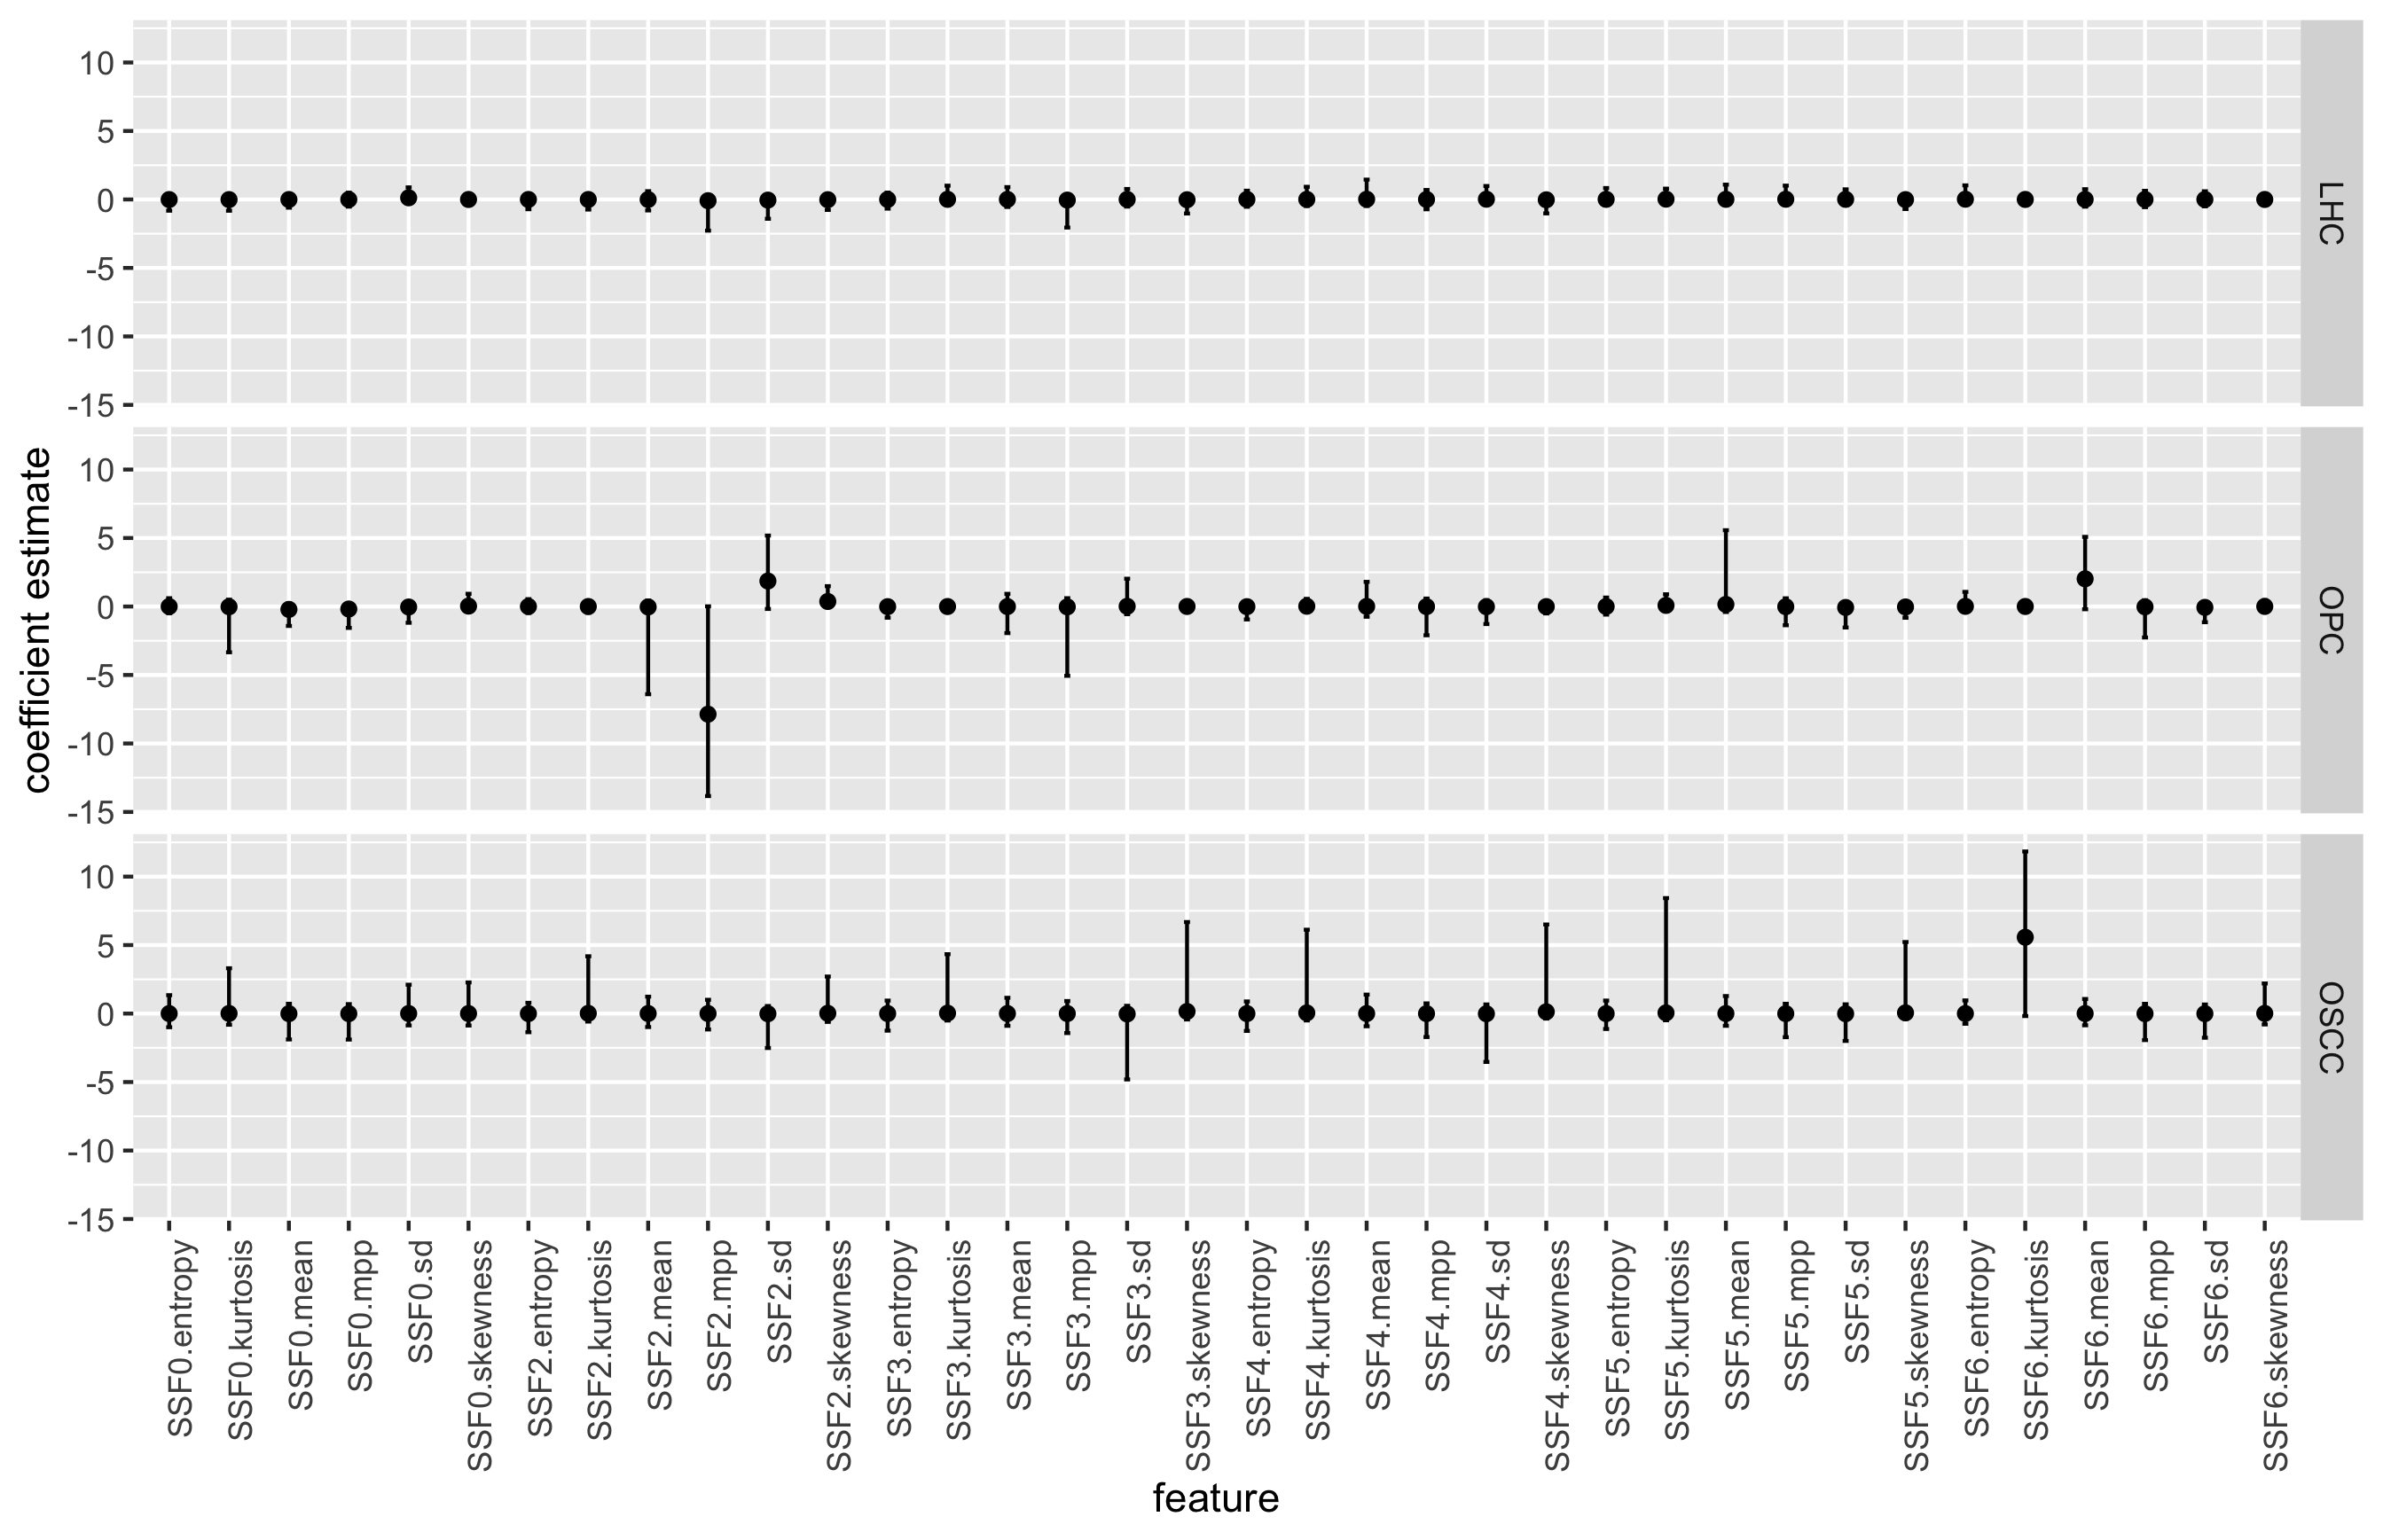
\includegraphics[width=\columnwidth]{mv_NS_feat.png}}
		\caption{Site-specific point estimates and 95\% credible intervals for the radiomic feature coefficients in the predictive model for lymph node metastasis}
		\label{fig1}
	\end{center}
\end{figure}

Prediction accuracy of the proposed model is illustrated in Figure~\ref{fig2} in form of 100 draws from the posterior distribution of the Receiver Operating Curves (ROC). The Area Under the Curve (AUC) varies from 0.81 to 0.84.



\begin{figure}[htbp]
	\begin{center}
		\centerline{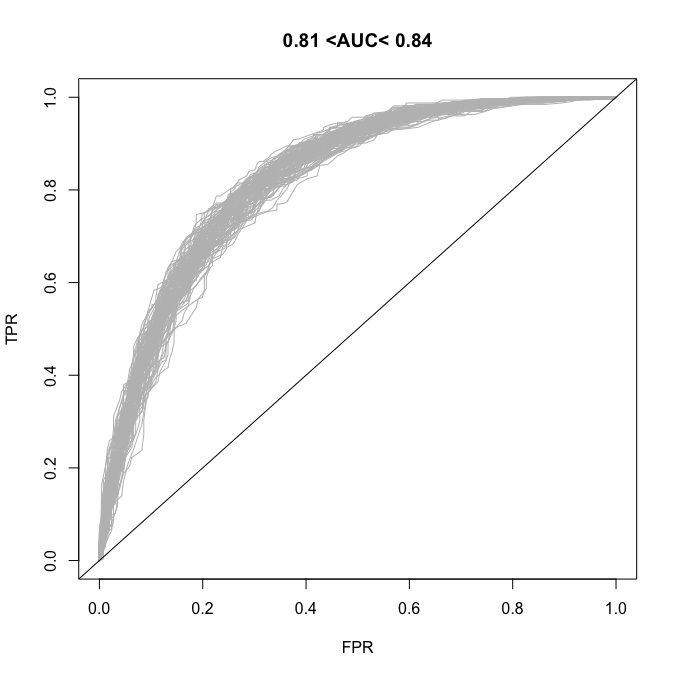
\includegraphics[width=0.9\columnwidth]{ROC.png}}
		\caption{Posterior draws from the Receiver Operating Curve for prediction of lymph node metastasis; The Area Under the Curve varies from 0.81 to 0.84.}
		\label{fig2}
	\end{center}
\end{figure}



\section{Discussion/Conclusions}

We have proposed a Bayesian hierarchical predictive model to analyse complex and high dimensional radiomic data. The novelty of the proposed model is in dealing with multiple challenging issues within a unified framework.  Namely, variable selection, missing data imputation and prediction are performed simultaneously within the proposed model. The main advantage of integrating variable (feature) selection and missing data handling together with estimation and prediction over multi-step procedures, is adequate representation of uncertainty in the final results. We further compared our apporach to popular machine learning techniques often used in the radiomics literature. For example, the random forest method applied to this data achieved an AUC of 0.76, but there was no way to obtain a site specific feature importance measure and HPV status was ignored in the training due to missingness. 
%*** Any comments regarding the performance in compare to existing methods? ***



\bibliographystyle{sdss2020} % Please do not change the bibliography style
\bibliography{SampleReferencesForExtendedAbstract}

\end{document}
